\documentclass{article}


% This file is a solution template for:
% 1 inch margins
\usepackage{fullpage}

\usepackage{booktabs}
\usepackage{longtable}

\usepackage{hyperref}
\usepackage{graphicx}
\usepackage{multicol}
\usepackage{subcaption}

% Add ability to resume enumeration environments with /begin{enumerate}[resume]
\usepackage{enumitem}

\usepackage{pgf}
\usepackage{tikz}
\usepackage{bodegraph}
\usepackage{circuitikz}
\usetikzlibrary{calc}
\usetikzlibrary{trees}
\usetikzlibrary{arrows}
\usetikzlibrary{shapes}
\usetikzlibrary{fadings}
\usetikzlibrary{positioning}
\usetikzlibrary{intersections}


\usepackage[english]{babel}
\usepackage[latin1]{inputenc}
\usepackage[T1]{fontenc}
% Or whatever. Note that the encoding and the font should match. If T1 does not look nice, try deleting the line with the fontenc.


\usepackage{listings}

\usepackage{amsmath}


\usepackage{xspace}
\newcommand{\Ohm}{$\Omega$\xspace}



\title{Diodes}


\begin{document}
\maketitle

This week we will explore another new passive circuit element, the diode. We will also explore some diode applications including conversion of an AC signal into a signal that never changes polarity. To go beyond this and make a real DC signal will take a few more tools including low-pass filters. 

\section{Theory}

\subsection{Nonlinear Devices}
The diode is our first nonlinear circuit element. A nonlinear element passes a current that is not proportional to the voltage across it (i.e. it does not obey Ohm's Law). Note, though, that a small change in the voltage across a diode will still generate a small change in its current. That is, if the change in voltage is small enough that the change in current will be proportional to that small voltage change. Thus, even circuits with diodes can use a Th\'{e}venin model for small deviations from the quiescent (or normal) condition of the circuit. 

\subsection{Diodes}
Diodes are an important component of a DC power supply since they can convert an alternating current to a direct current. Most of the time, we will model a diode as simply a one-way gate for current. 

In most wires and resistors, current is carried exclusively by electrons, which have negative charge. Semiconductors (silicon based devices) can use either negative charge carriers (electrons) or positively charged carriers (called holes) depending on what impurities have been added to the silicon when it was grown into a crystal. One type of impurity (called n doping) creates the negative carriers, and the other type of impurity (called p doping) creates positive carriers. A junction between p-doped and n-doped silicon makes a diode. Electrons and holes can easily recombine with each other at a pn junction producing a net current flow from p to n. However, if the current wants to flow in the other direction, so that both electrons and holes move away from the junction, then the junction will act like an open switch. Thus, diodes are simple devices with the remarkable property that they only conduct current in one direction.

\subsection{Diode Model 1: The Current Gate}
\begin{figure}
\begin{center}
\begin{circuitikz}
\draw (0,0) node[ground]{} to[battery1,l=$V_{in}$] (0,2) to[diode] (2,2) to[R,l=$R$] (2,0) node[ground]{};
\draw (2,2) to[short,-o] (3,2) node[right]{$V_{out}$};
\end{circuitikz}
\end{center}
\caption{The diode acts as a one-way current gate.}
\label{fig:current-gate}
\end{figure}

For almost all practical purposes, we will treat a diode as a one-way current gate that also produces a 0.6\,V voltage drop for silicon and 0.2\,V drop for germanium. The voltage drop is due to the energy converted to heat as the electron-hole pair recombines. Diodes have a marking on them (sometimes just the line at the output end), showing the direction they conduct. In the accompanying figure, the diode will only conduct if $V_{in} > 0.6$\,V. When the diode does conduct, any excess voltage drop shows up across the resistor. In other words, the diode just conducts enough current to set I such that 
\begin{equation}
I R = V_{in} - 0.6\,\hbox{V}
\end{equation}

\subsection{Diode Model 2: The Ebers-Moll Model}
A more complete model of a diode would treat the resistance of the diode as a logarithm of the voltage applied. In this more complete model, shown graphically in Figure~\ref{fig:diode-IV-characteristic} below, we note that the 0.6\,V threshold is only an approximation for reasonable voltages. 

\begin{figure}
\begin{center}
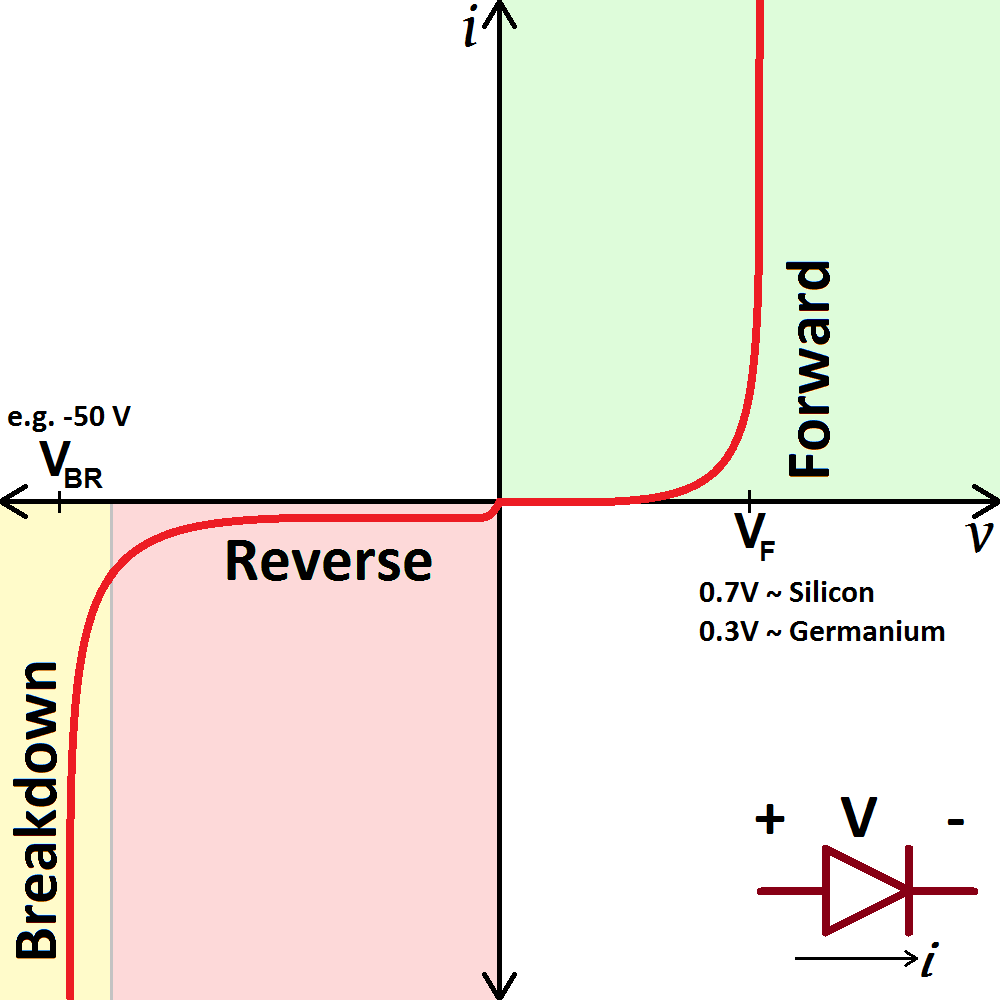
\includegraphics[width=0.45\textwidth]{pics/diode_IV_characteristic}
\end{center}
\caption{A typical silicon diode I-V characteristic curve with forward, reverse, and breakdown regions indicated. [Image credit: \href{https://learn.sparkfun.com/tutorials/diodes/real-diode-characteristics}{Sparkfun}]}
\label{fig:diode-IV-characteristic}
\end{figure}

The I-V characteristic of a diode is given by the Ebers-Moll equation of solid state physics:
\begin{equation}
I = I_0 \left(e^{\frac{V}{V_T}} - 1\right)
\end{equation}
where for silicon at room temperature the reverse saturation current $I_0 = 10^{-9}$\,A, and the thermal voltage $V_T = \frac{kT}{e} = 25.3$\,mV. This equation is valid in both the forward bias and the reverse bias regions, but does not apply in the breakdown region. Real diodes generally exhibit small deviations from this model.

\section{Some Applications}
Diodes have many applications. Here are a few of them.

\subsection{Diode Rectifiers}
\paragraph{Half-wave rectifier}
\begin{figure}
\begin{center}
\begin{circuitikz}
\draw (0,0) node[ground]{} to[sV,l=$V_{in}$] (0,2) to[diode] (2,2) to[R,l=$R$] (2,0) node[ground]{};
\draw (2,2) to[short,-o] (3,2) node[right]{$V_{out}$};
\end{circuitikz}
\end{center}
\caption{A half-wave rectifier only passes the positive input voltages to the output.}
\label{fig:half-wave-rectifier}
\end{figure}
One of the most common uses for diode is to rectify AC voltage to make a DC power supply. Since a single diode can only conduct current one way, when the input wave goes negative, there will be no current, as in the half-wave rectifier circuit of Figure~\ref{fig:half-wave-rectifier}.

\paragraph{Full-wave rectifier}
\begin{figure}
\begin{center}
\begin{circuitikz}
\draw (0,2) node[right]{$V_{in}^+$} to[short,o-] (0,1.5);
\draw (0,-2) node[right]{$V_{in}^-$} to[short,o-] (0,-1.5);
\draw (-1.5,0) to[diode] (0,1.5) to[diode] (1.5,0);
\draw (-1.5,0) to[diode] (0,-1.5) to[diode] (1.5,0);
\draw (1.5,0) to[short] (2,0) to[short,-o] (2.5,0) node[right]{$V_{out}^+$};
\draw (-1.5,0) to[short] (-2,0) to[short] (-2,-3) to[short] (2,-3) to[short,-o] (2.5,-3) node[right]{$V_{out}^-$};
\draw (2,0) to[R] (2,-3);
\end{circuitikz}
\end{center}
\caption{A full-wave rectifier passes the positive input voltages and inverts the negative input voltages.}
\label{fig:full-wave-rectifier}
\end{figure}
With four diodes, you can make both halves of the waves positive. This is called a full-wave rectifier diode bridge and is shown in Figure~\ref{fig:full-wave-rectifier} on the right. For both positive and negative swings of the input there is a forward path through the diode bridge. While two of the diodes are forward biased, the other two are reverse biased and effectively eliminated from the circuit. Both conduction paths cause current to flow in the same direction through the load resistor, accomplishing full-wave rectification.

Full-wave rectifiers are used in power supplies to convert AC voltages to DC voltages (or at least ones which are positive). A large capacitor in parallel with the output load resistor reduces the  ripple from the rectification process.

\subsection{Frequency multipliers}
A full-wave rectifier is also a frequency multiplier. The output of a rectified 60\,Hz signal is at 120\,Hz, but also has components at 240\,Hz, 360\,Hz,\ldots as is shown in Figure~\ref{fig:frequency-multiplier}.

\begin{figure}
 \begin{center}
  \begin{subfigure}[b]{0.48\textwidth}
   \begin{center}
    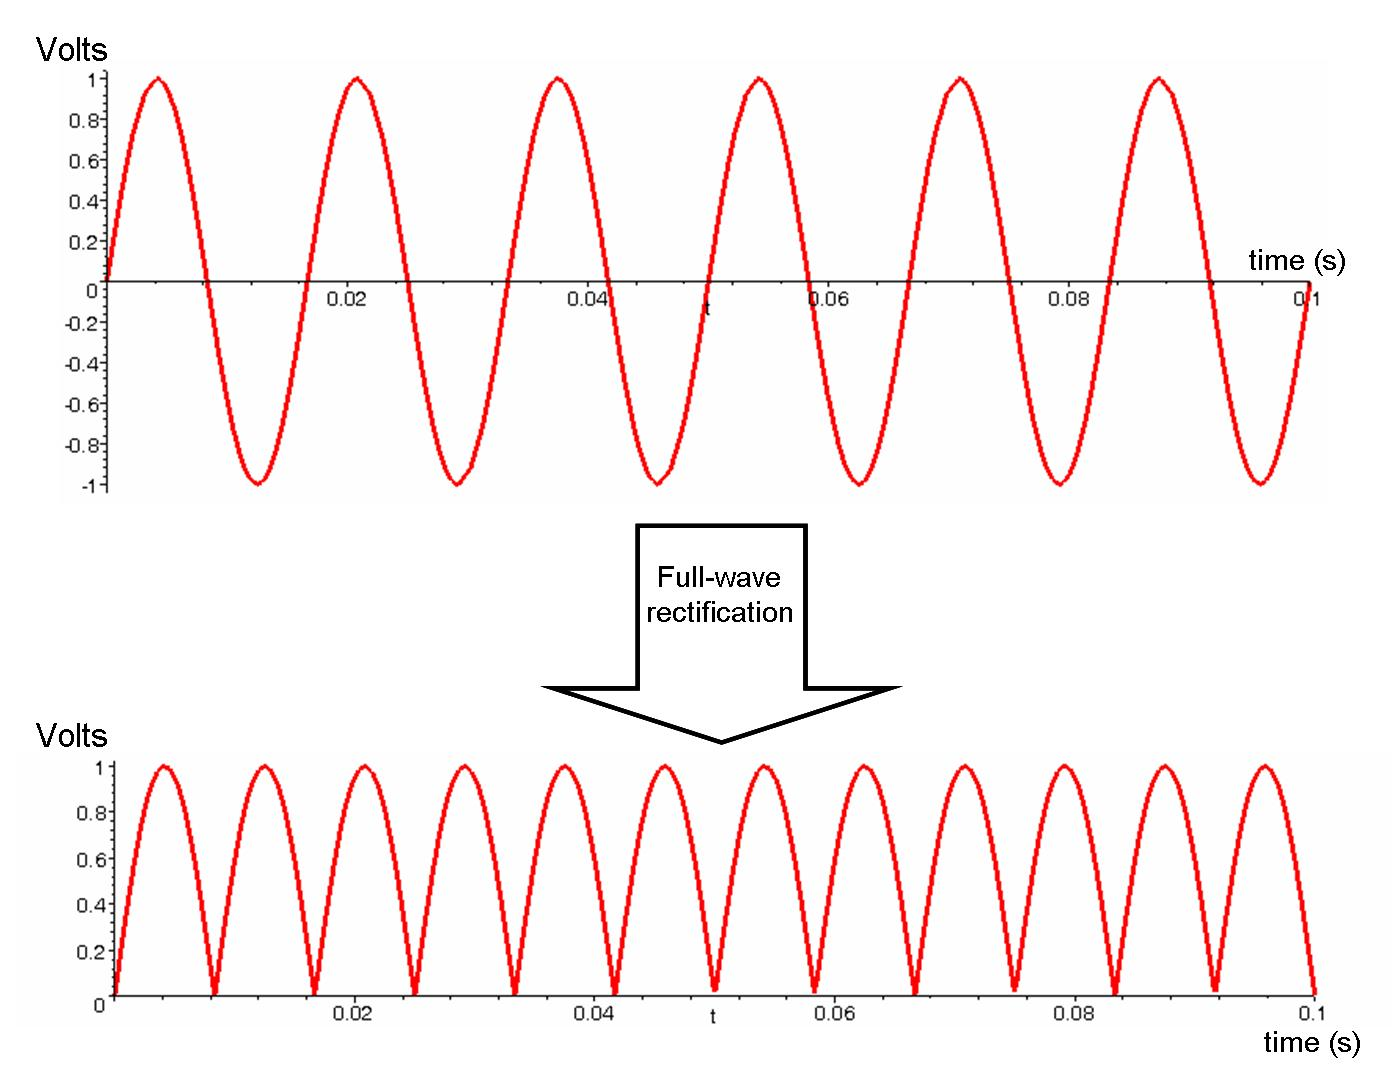
\includegraphics[width=\textwidth]{pics/frequency_multiplier_time}
   \end{center}
   \caption{time domain}
  \end{subfigure}
  \begin{subfigure}[b]{0.48\textwidth}
   \begin{center}
    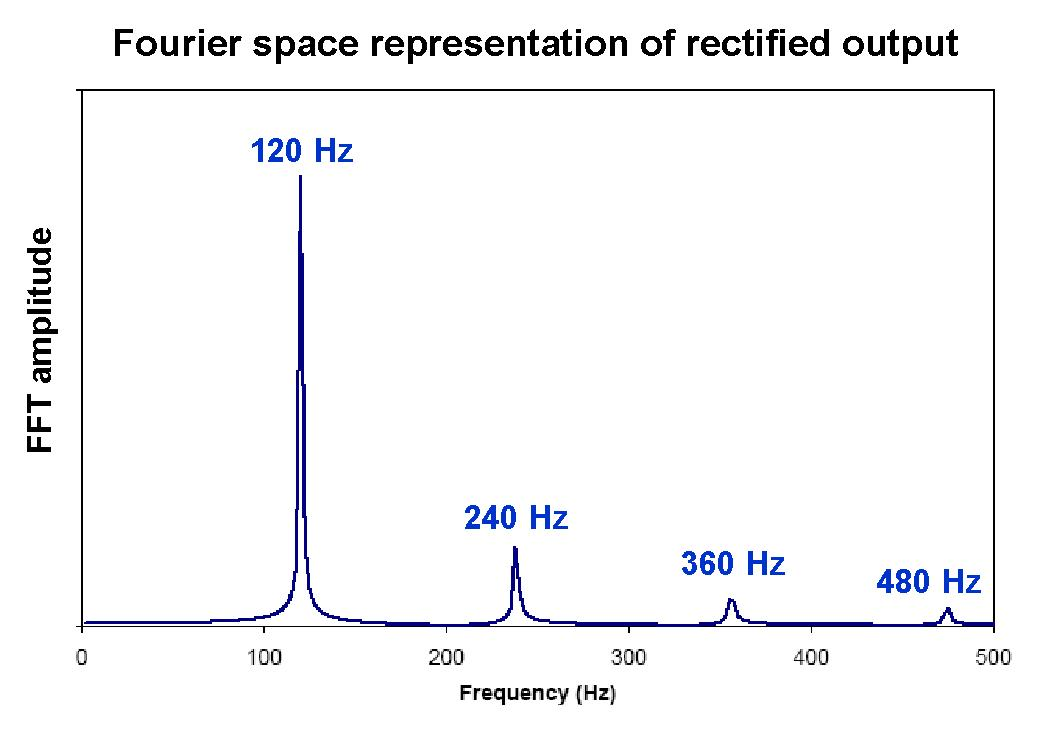
\includegraphics[width=\textwidth]{pics/frequency_multiplier_FFT}
   \end{center}
   \caption{frequency domain}
  \end{subfigure}
 \end{center}
\caption{The ideal performance of a full-wave rectifier results in a doubling of the input frequency.}
\label{fig:frequency-multiplier}
\end{figure}

In the above Fourier space representation, we have not included the zero frequency component (i.e. the DC bias) in the plot.

Filtering after the full-wave rectifier is used to remove the unwanted harmonics.

\subsection{Frequency Mixers}
A full-wave rectifier can also be used as a frequency mixer when two frequencies, $f_1$ and $f_2$ are input simultaneously into the full-wave rectifier: the output will include frequencies at $|f_1-f_2|$ and $f_1+f_2$, in addition to the harmonics of $2f_1$ and $2f_2$.


\pagebreak

\section{Lab 5: Design Exercises}
\begin{enumerate}
\item Design a 12\,V DC power supply out of a standard US AC line source (120\,V AC, 60\,Hz).  Do the above quote 120\,V AC refer to amplitude, RMS, or peak-to-peak voltage? Use some diodes, a transformer and a low pass filter (i.e. a large capacitor). You need to calculate the desired transformer coils ratio (do not forget about the diode voltage drop). The ripple voltage at the output of your supply should not exceed 0.1\,V when it has a 1\,k\Ohm load. 
\end{enumerate}

\section{Lab 5: Diodes}

\subsection{I-V Characteristic of a Diode (estimated time: 30 minutes\ldots 1 hour)}
\begin{enumerate}
\item Measure the I-V characteristic of a diode (you may use a regular diode or an LED). Please make sure that you do not exceed ~100\,mA though the diode. A good way to measure the I-V curve is to use the ``one-way current gate'' circuit from the course notes so that the resistor (100\,\Ohm recommended) limits the current flowing through the circuit. Also, try to keep your circuit components close to room temperature since their performance will change if they heat up. Do not use multimeters for the current measurements.
\end{enumerate}

\subsection{Full-Wave Rectifier (estimated time: 30 minutes)}
\label{lab:full-wave-rectifier}
\begin{enumerate}
\item Construct the full-wave rectifier with a voltage signal at 1\,kHz, four diodes, an audio transformer, and a load resistor of 100\,k\Ohm. Use a signal generator with a 2\,V peak-to-peak output and connect it to the transformer in step up fashion.
\item Measure the amplitude of the signal after transformer and characterize the output signal through the load resistor. Sketch the voltage across the load resistor and measure the size of the ripples.
\item For two different filtering capacitors ($6.8\,\mu$F and 10\,nF) connected in parallel to the load, sketch or save scope traces at the output and measure the size of the ripples.
%\item Change the signal generator voltage level such that the output after the filtering capacitor is positive and between 7.5\,V and 9\,V.  Connect an LM7805 voltage regulator according to the datasheet and measure the remaining ripples in the output voltage.
\item By the way, why do we need the transformer?
\end{enumerate}

\subsection{Frequency Multiplier (estimated time: 30 minutes)}
\begin{enumerate}
\item Use the same set-up as lab assignment~\ref{lab:full-wave-rectifier} but remove the filtering capacitor.  Use the FFT (Fast Fourier Transform) function to measure the frequency spectrum of the output. Measure the amplitude and frequency of the principal harmonics (i.e. the one you can see). How do you convert dB to Volts? What FFT window did you use? Does it matter?
\end{enumerate}

\end{document}
